\documentclass[border=6pt]{standalone}
\usepackage{tikz}
\usetikzlibrary{arrows.meta,positioning}
\begin{document}
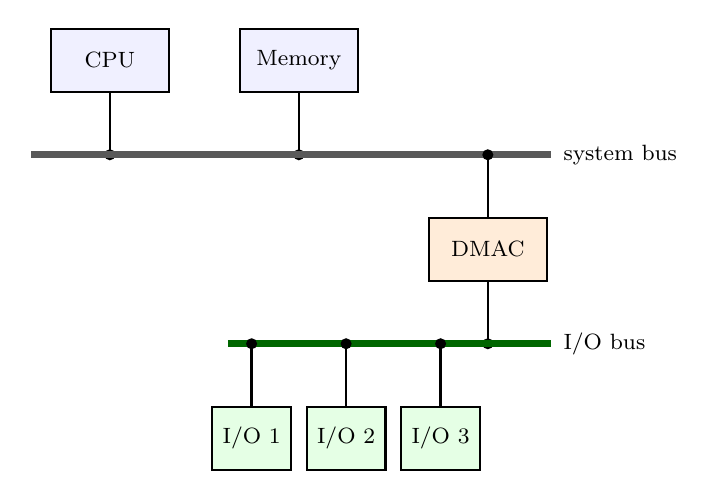
\begin{tikzpicture}[font=\small,
 m/.style={draw,thick,fill=blue!6,minimum width=1.5cm,minimum height=0.8cm,align=center,font=\footnotesize}]
\node[m] at (0,1.2) {CPU}; \draw[thick] (0,0.8) -- (0,0); \fill (0,0) circle (2pt);
\node[m] at (2.4,1.2) {Memory}; \draw[thick] (2.4,0.8) -- (2.4,0); \fill (2.4,0) circle (2pt);
\draw[line width=2.5pt,gray!70!black] (-1.0,0) -- (5.6,0) node[right,font=\footnotesize,black]{system bus};
\node[m,fill=orange!15] at (4.8,-1.2) {DMAC};
\draw[thick] (4.8,-0.8) -- (4.8,0); \fill (4.8,0) circle (2pt);
\draw[thick] (4.8,-1.6) -- (4.8,-2.4); \fill (4.8,-2.4) circle (2pt);
\draw[line width=2.5pt,green!40!black] (1.5,-2.4) -- (5.6,-2.4) node[right,font=\footnotesize,black]{I/O bus};
\foreach \x/\n in {1.8/1,3.0/2,4.2/3} {
  \node[m,fill=green!10,minimum width=1.0cm] at (\x,-3.6) {I/O \n};
  \draw[thick] (\x,-3.2) -- (\x,-2.4); \fill (\x,-2.4) circle (2pt);
}
\end{tikzpicture}
\end{document}
